\reviewexercisesheader{}

% 1

\eoce{\qt{Multiple regression fact checking\label{mult_regr_facts}}
Determine which of the following statements are
true and false.
For each statement that is false, explain why it is false.
\begin{parts}
\item
    If predictors are collinear, then removing
    one variable will have no influence on the
    point estimate of another variable's coefficient.
\item
    Suppose a numerical variable $x$ has a coefficient of
    $b_1 = 2.5$ in the multiple regression model.
    Suppose also that the first observation has $x_1 = 7.2$,
    the second observation has a value of $x_1 = 8.2$,
    and these two observations have the same values
    for all other predictors.
    Then the predicted value of the second observation
    will be 2.5 higher than the prediction of the first
    observation based on the multiple regression model.
\item
    If a regression model's first variable has
    a coefficient of $b_1 = 5.7$, then if we are
    able to influence the data so that an observation
    will have its $x_1$ be 1 larger than it would
    otherwise, the value $y_1$ for this observation
    would increase by 5.7.
\item
    Suppose we fit a multiple regression model
    based on a data set of 472 observations.
    We also notice that the distribution of the
    residuals includes some skew but does not
    include any particularly extreme outliers.
    Because the residuals are not nearly normal,
    we should not use this model and require
    more advanced methods to model these data.
\end{parts}
}{}

% 2

\eoce{\qt{Logistic regression fact checking\label{log_regr_facts}}
Determine which of the following statements are
true and false.
For each statement that is false, explain why it is false.
\begin{parts}
\item
    Suppose we consider the first two observations
    based on a logistic regression model,
    where the first variable in observation~1
    takes a value of $x_1 = 6$ and observation~2
    has $x_1 = 4$.
%    Each observation has all the same values for the
%    other variables used in the model.
    Suppose we realized we made an error for these
    two observations, and the first observation
    was actually $x_1 = 7$ (instead of~6)
    and the second observation actually had
    $x_1 = 5$ (instead of~4).
    Then the predicted probability from the
    logistic regression model would increase
    the same amount for each observation after
    we correct these variables.
\item
    When using a logistic regression model,
    it is impossible for the model to predict
    a probability that is negative or a probability
    that is greater than 1.
\item
    Because logistic regression predicts probabilities
    of outcomes, observations used to build a logistic
    regression model need not be independent.
\item
    When fitting logistic regression,
    we typically complete model selection using
    adjusted $R^2$.
\end{parts}
}{}

% 3

\eoce{\qt{Spam filtering, Part I\label{spam_filtering_model_sel}}
Spam filters are built on principles similar to those
used in logistic regression.
We fit a probability that each message is spam
or not spam.
We have several email variables for this problem:
\resp{to\us{}multiple},
\resp{cc},
\resp{attach},
\resp{dollar},
\resp{winner},
\resp{inherit},
\resp{password},
\resp{format},
\resp{re\us{}subj},
\resp{exclaim\us{}subj}, and
\resp{sent\us{}email}.
We won't describe what each variable means
here for the sake of brevity, but each is
either a numerical or indicator variable.
\begin{parts}
\item
    For variable selection,
    we fit the full model, which includes all
    variables, and then we also fit each model
    where we've dropped exactly one of the variables.
    In each of these reduced models, the AIC value
    for the model is reported below.
    Based on these results, which variable,
    if any, should we drop as part of model
    selection?
    Explain.
    \begin{center}
    \begin{tabular}{lc}
      \hline
      Variable Dropped & AIC \\ 
      \hline
      None Dropped & 1863.50 \\ 
      \resp{to\us{}multiple} & 2023.50 \\ 
      \resp{cc} & 1863.18 \\ 
      \resp{attach} & 1871.89 \\ 
      \resp{dollar} & 1879.70 \\ 
      \resp{winner} & 1885.03 \\ 
      \resp{inherit} & 1865.55 \\ 
      \resp{password} & 1879.31 \\ 
      \resp{format} & 2008.85 \\ 
      \resp{re\us{}subj} & 1904.60 \\ 
      \resp{exclaim\us{}subj} & 1862.76 \\ 
      \resp{sent\us{}email} & 1958.18 \\ 
      \hline
    \end{tabular}
    \end{center}

\item
    Consider the following version of the model.
    Here again we've computed the AIC
    for each leave-one-variable-out model.
    Based on the results, which variable,
    if any, should we drop as part of model
    selection?
    Explain.
    \begin{center}
    \begin{tabular}{lc}
      \hline
      Variable Dropped & AIC \\ 
      \hline
      None Dropped & 1862.41 \\ 
      \resp{to\us{}multiple} & 2019.55 \\ 
      \resp{attach} & 1871.17 \\ 
      \resp{dollar} & 1877.73 \\ 
      \resp{winner} & 1884.95 \\ 
      \resp{inherit} & 1864.52 \\ 
      \resp{password} & 1878.19 \\ 
      \resp{format} & 2007.45 \\ 
      \resp{re\us{}subj} & 1902.94 \\ 
      \resp{sent\us{}email} & 1957.56 \\ 
      \hline
    \end{tabular}
    \end{center}
\end{parts}
}{}

% 4

\eoce{\qt{Movie returns, Part II\label{movie_returns_by_genre}}
The student from
Exercise~\ref{movie_returns_altogether} analyzed
return-on-investment (ROI) for movies based on
release year and genre of movies.
The plots below show the predicted ROI vs. actual
ROI for each of the genres separately.
Do these figures support the comment in the
FiveThirtyEight.com article that states,
``The return-on-investment potential for horror movies
is absurd.''
Note that the x-axis range varies for each plot.
\begin{center}
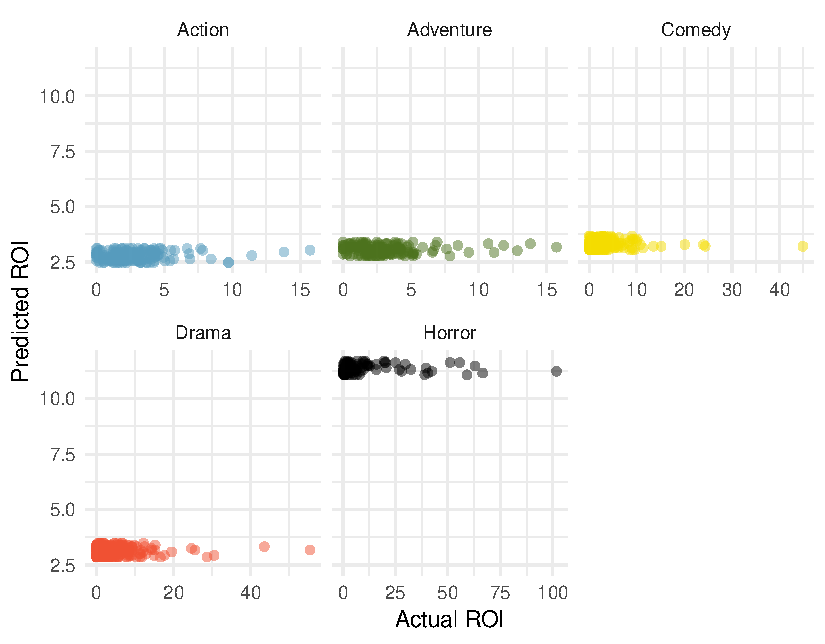
\includegraphics[width=0.6\textwidth]{ch_regr_mult_and_log/figures/eoce/movie_returns_by_genre/horror_movies_by_genre}
\end{center}
}{}

% 5

\eoce{\qt{Spam filtering, Part II\label{spam_filtering_predict}}
In Exercise~\ref{spam_filtering_model_sel},
we encountered a data set where we applied
logistic regression to aid in spam classification
for individual emails.
In this exercise, we've taken a small set of these
variables and fit a formal model with the following
output:
\begin{center}
\begin{tabular}{rrrrr}
  \hline
  & Estimate & Std. Error & z value & Pr($>$$|$z$|$) \\ 
  \hline
  (Intercept) & -0.8124 & 0.0870 & -9.34 & 0.0000 \\ 
  to\us{}multiple & -2.6351 & 0.3036 & -8.68 & 0.0000 \\ 
  winner & 1.6272 & 0.3185 & 5.11 & 0.0000 \\ 
  format & -1.5881 & 0.1196 & -13.28 & 0.0000 \\ 
  re\us{}subj & -3.0467 & 0.3625 & -8.40 & 0.0000 \\ 
  \hline
\end{tabular}
\end{center}
\begin{parts}
\item
    Write down the model using the coefficients
    from the model fit.

\item
    Suppose we have an observation where
    $\var{to\us{}multiple} = 0$,
    $\var{winner} = 1$,
    $\var{format} = 0$, and
    $\var{re\us{}subj} = 0$.
    What is the predicted probability that this message
    is spam?

\item
    Put yourself in the shoes of a data scientist
    working on a spam filter.
    For a given message, how high must the probability
    a message is spam be before you think it would be
    reasonable to put it in a \emph{spambox}
    (which the user is unlikely to check)?
    What tradeoffs might you consider?
    Any ideas about how you might make your spam-filtering
    system even better from the perspective of someone
    using your email service?
\end{parts}
}{}
